\begin{slide}{Math. Grundlagen d. Informatik (Uni Halle)}

\begin{itemize}
\item
  Mengen und algebraische Strukturen

  \emph{Mengenoperationen}  (Algebraic-Set)
  \\  \emph{Verkn�pfungen von Relationen}  (Algebraic-Relation)
  \\ \emph{mehrsortige Algebren} (Sorten)
\item
  Graphen
  
  \emph{Circle}, \emph{Wegematrix} (Way), \emph{Bitpartit} (Bi),
  \\ \emph{F�rbung} (Col), \emph{Hamilton} 
  \\ \emph{Selbstkomplement�rer Graph}, \emph{Nachbar}
  \\ \emph{Operationen auf Graphen} (Algebraic-Graph)
\end{itemize}

\end{slide}
%% -----------------------------------------------------
\begin{slide}{Logik}

\begin{itemize}
\item
  Aussagenlogik

  \emph{erf�llende Belegung} (SAT)
  \\ \emph{�quivalente boolesche Ausdr�cke} (Boolean)
  \\ \emph{Beweise im Hilbert-Kalk�l} (Hilbert)
\item
  Pr�dikatenlogik
  
  \emph{Modelle f�r Formeln} (Find-Model)
\end{itemize}

\end{slide}
%% -----------------------------------------------------
\begin{slide}{Mengenoperationen}
\begin{verbatim}  
Gesucht ist ein Ausdruck mit dieser Bedeutung:
{1, 5, {}, {4}}
Sie d�rfen diese Symbole benutzen
    zweistellige : [ + , - , & ]
    einstellige  : [ pow ]
    nullstellige : [ 0 , 1 , 2 , 3 , 4 , 5 , 6]
und diese vordefinierten Konstanten:
    A = {1, 3, 5, 6}
    B = {2, 3, 6}
\end{verbatim}

L�sung: \begin{verbatim}  A - B + pow (4)  \end{verbatim}
\end{slide}
%% -----------------------------------------------------
\begin{slide}{Relationen}
\begin{verbatim}
Gesucht ist ein Ausdruck mit dieser Bedeutung:
   {(2 , 3) , (4 , 1)}
Sie d�rfen diese Symbole benutzen
    zweistellige : [ + , - , & , * ]
    einstellige  : [ inv , tcl , rcl ]
    nullstellige : [ ]
und diese vordefinierten Konstanten:
    R = {(1 , 2) , (3 , 4)}
    S = {(2 , 3) , (4 , 1) , (5 , 2)}
\end{verbatim}

L�sung: \begin{verbatim}  inv (R * S * R) \end{verbatim}

\end{slide}
%% -----------------------------------------------------
\begin{slide}{Operationen auf Graphen}
{\small 
\begin{verbatim}  
Gesucht ist ein Ausdruck mit dieser Bedeutung:
\end{verbatim}
\begin{minipage}{0.4\textwidth}
\includegraphics[width=4cm]{mathgrundbild.eps}
\end{minipage}%

\begin{verbatim}  
der nur diese Symbole enth�lt:
    Binu { binary = [ * , % , + ] , unary = [ co ]
         , nullary = [ K1 , K2 , K3 , K4 , K5 , P3 , P4 , P5 
                      , C3 , C4 , C5] }
\end{verbatim}

L�sung: \begin{verbatim} C5 % P3 \end{verbatim}
}
\end{slide}
%% -----------------------------------------------------
\begin{slide}{Hilbert-Kalk�l}
{\small
\begin{verbatim}
Gesucht ist eine Ableitung f�r die Formel
    p -> p
im Hilbert-Kalk�l mit den Axiomen
    { H1 = A -> (B -> A)
    , H2 = (A -> (B -> C)) -> ((A -> B) -> (A -> C))
    , H3 = (A -> B) -> (not B -> not A) , H4 = A -> (not A -> B)
    , H5 = (not A -> A) -> A
    }
\end{verbatim}
L�sung:
\begin{verbatim}
let { F1 = sub H1 { A = p , B = q -> p }
    , F2 = sub H2 { A = p , B = q -> p, C = p}
    , F3 = mopo F1 F2
    , F4 = sub H1 { A = p, B = q}}
in mopo F4 F3
\end{verbatim}
}
\end{slide}
%% -----------------------------------------------------
\begin{slide}{Modelle (Pr�dikatenlogik)}
{\small
\begin{verbatim}
Finden Sie f�r die Formel
    forall x . exists y. R (x , y) && (not P (y))
ein Modell (eine Interpretation) der Gr��e
    3
\end{verbatim}

L�sung: \begin{verbatim} 
Interpretation { struktur = 
Struktur { universum = mkSet [ 1 , 2, 3]
         , predicates = listToFM [ ( P , {} ) 
                , ( R , {(1,1), (2,2), (3,1)} ) ]
         , functions = listToFM [ ]}
         , belegung = listToFM [ ] 
         } 
\end{verbatim}
}
\end{slide}
